\section{Results}

This section presents results of the conducted experiments, mostly in the form of tables and line plots. Tables show average testing performance over the 5 trials per experiment, with standard deviation ($s$) between brackets. A green shaded cell marks best performance, while yellow and red depict second best and worst performance, respectively.

Line plots mostly show average validation accuracy (dashed line is CNN-based, continuous is ViT-based), with \textit{standard error of the mean} ($\pm s \div \sqrt{N}$, where $N=5$) depicted as a shaded region. Plots end when an early stop occurred for the first of 5 trials.

% Tell that the appendix shows all other plots as well maybe. Only for the BP paper tho.


\subsection{Off the shelf learning} \label{results:ots}

\begin{figure*}
    \centering
    \begin{subfigure}{0.32\textwidth}
    \def\svgwidth{5.5cm}
    \input{img/ots_type_acc.pdf_tex}
    \caption{Type}
    \label{results:img:ots_type}
    \end{subfigure}
    \hfill
    \begin{subfigure}{0.32\textwidth}
    \def\svgwidth{5.5cm}
    \input{img/ots_mat_acc.pdf_tex}
    \caption{Material}
    \label{results:img:ots_mat}
    \end{subfigure}
    \hfill
    \begin{subfigure}{0.32\textwidth}
    \def\svgwidth{5.5cm}
    \input{img/ots_artist_acc.pdf_tex}
    \caption{Artist}
    \label{results:img:ots_artist}
    \end{subfigure}
    \caption{Validation accuracy using off the shelf models.}
    \label{results:img:ots}
\end{figure*}

\begin{table}[tb]
\resizebox{\columnwidth}{!}{%
\begin{tabular}{lll}
\hline
\textbf{Model} & \textbf{Accuracy} & \textbf{Balanced accuracy} \\ \hline
\textbf{vit\_b\_16} & 86.06\% (${\pm 1.06\%}$) & 84.13\% (${\pm 1.57\%}$)  \\
\textbf{swin\_b} & \cellcolor{bestcol}89.43\% (${\pm 0.93\%}$) & \cellcolor{bestcol}87.47\% (${\pm 1.02\%}$)  \\
\textbf{beit\_b\_16} & \cellcolor{worstcol}82.26\% (${\pm 0.72\%}$) & \cellcolor{worstcol}77.75\% (${\pm 0.27\%}$)  \\
\textbf{deit\_b\_16} & 88.18\% (${\pm 0.66\%}$) & 85.36\% (${\pm 0.54\%}$)  \\\hdashline
\textbf{vgg19} & 83.93\% (${\pm 0.72\%}$) & 83.35\% (${\pm 0.81\%}$)  \\
\textbf{resnet50} & 85.51\% (${\pm 0.64\%}$) & 82.33\% (${\pm 1.85\%}$)  \\
\textbf{efficientnetv2\_m} & 83.41\% (${\pm 0.76\%}$) & 82.05\% (${\pm 1.25\%}$)  \\
\textbf{convnext\_b} & \cellcolor{secondbestcol}89.19\% (${\pm 0.64\%}$) & \cellcolor{secondbestcol}86.95\% (${\pm 1.38\%}$)  \\\hline
\end{tabular}
}
\caption{Type classification off the shelf}
\label{results:tab:ots_type}
\end{table}


\begin{table}[tb]
\resizebox{\columnwidth}{!}{%
\begin{tabular}{lll}
\hline
\textbf{Model} & \textbf{Accuracy} & \textbf{Balanced accuracy} \\ \hline
\textbf{vit\_b\_16} & 81.78\% (${\pm 0.48\%}$) & 67.38\% (${\pm 1.37\%}$)  \\
\textbf{swin\_b} & \cellcolor{bestcol}85.87\% (${\pm 0.35\%}$) & \cellcolor{bestcol}71.19\% (${\pm 1.60\%}$)  \\
\textbf{beit\_b\_16} & 76.87\% (${\pm 0.96\%}$) & 60.16\% (${\pm 1.56\%}$)  \\
\textbf{deit\_b\_16} & 82.80\% (${\pm 1.12\%}$) & 66.46\% (${\pm 1.03\%}$)  \\\hdashline
\textbf{vgg19} & 76.87\% (${\pm 0.44\%}$) & 61.39\% (${\pm 1.47\%}$)  \\
\textbf{resnet50} & 80.99\% (${\pm 0.82\%}$) & 65.51\% (${\pm 0.93\%}$)  \\
\textbf{efficientnetv2\_m} & \cellcolor{worstcol}75.96\% (${\pm 1.24\%}$) & \cellcolor{worstcol}59.15\% (${\pm 1.24\%}$)  \\
\textbf{convnext\_b} & \cellcolor{secondbestcol}84.14\% (${\pm 0.92\%}$) & \cellcolor{secondbestcol}69.10\% (${\pm 1.05\%}$)  \\\hline
\end{tabular}
}
\caption{Material classification off the shelf}
\label{results:tab:ots_mat}
\end{table}


\begin{table}[tb]
\resizebox{\columnwidth}{!}{%
\begin{tabular}{lll}
\hline
\textbf{Model} & \textbf{Accuracy} & \textbf{Balanced accuracy} \\ \hline
\textbf{vit\_b\_16} & 84.89\% (${\pm 0.46\%}$) & 81.42\% (${\pm 0.42\%}$)  \\
\textbf{swin\_b} & \cellcolor{bestcol}90.40\% (${\pm 0.65\%}$) & \cellcolor{bestcol}88.64\% (${\pm 0.78\%}$)  \\
\textbf{beit\_b\_16} & 79.70\% (${\pm 0.69\%}$) & 75.35\% (${\pm 1.09\%}$)  \\
\textbf{deit\_b\_16} & 88.13\% (${\pm 0.76\%}$) & 85.62\% (${\pm 0.87\%}$)  \\\hdashline
\textbf{vgg19} & 82.01\% (${\pm 0.66\%}$) & 78.10\% (${\pm 0.77\%}$)  \\
\textbf{resnet50} & 87.71\% (${\pm 1.06\%}$) & 85.12\% (${\pm 1.34\%}$)  \\
\textbf{efficientnetv2\_m} & \cellcolor{worstcol}78.62\% (${\pm 1.07\%}$) & \cellcolor{worstcol}73.92\% (${\pm 0.96\%}$)  \\
\textbf{convnext\_b} & \cellcolor{secondbestcol}90.13\% (${\pm 0.94\%}$) & \cellcolor{secondbestcol}87.84\% (${\pm 1.07\%}$)  \\\hline
\end{tabular}
}
\caption{Artist classification off the shelf}
\label{results:tab:ots_artist}
\end{table}


Tables \ref{results:tab:ots_type} through \ref{results:tab:ots_artist} show testing performance of OTS trained models on the 3 classification tasks, while figure \ref{results:img:ots} shows corresponding validation accuracies. Performance on the testing set is comparable among all tasks in terms of ranking. Other observations are consistent as well, such as ConvNext taking the longest to converge.

Swin is coming out on top in all cases, which is in line with results of \citeauthor{zhou2021convnets} (\citeyear{zhou2021convnets}). What slightly deviates from these result, is the observation that ViT performs better than a ResNet-based model (on 2 out of 3 tasks). This comparison is, however, not meaningful, as \citeauthor{zhou2021convnets} uses ResNet101 and 152. Using these models instead, gives 86.21\% ($\pm$ 0.70\%) accuracy for ResNet101, and 86.19\% ($\pm$ 0.60\%) for ResNet152, which is indeed slightly higher than ViT's 86.06\% shown in table \ref{results:tab:ots_type}.

It is interesting that VGG19 performs worse than ResNet50, since it was the best performing OTS model on all 3 tasks in \citeauthor{sabatelli2018deep} (\citeyear{sabatelli2018deep}). The current study uses smaller datasets and fewer classes. The difference might be attributable to this, as VGG19 is the largest model (see section \ref{methods:models}), and has the largest final layer -- with 4096 inputs.

When comparing tasks to one another, it can be observed that overall accuracies are lowest for material classification, and highest for artist classification. In addition, the difference between balanced and plain accuracy is the largest for material classification (up to 14\% on the testing set), while it is the smallest for artist classification (at most 4.7\%). Note that Gini-coefficients in table \ref{methods:datasets} show the same trend, with material classification being the least balanced, and artist classification the most.

As a whole, ViTs are doing well for the OTS experiments. Especially Swin and DeiT are ranked high on all testing sets, while ConvNext is the most promising CNN-based architecture. Taking the mean accuracy of all ViT- and CNN-based models, reveals that ViTs as a group perform slightly better. On type classification, for example, their mean accuracy is 86.5\%, while it is 85.5\% for CNNs.

% This seems counterintuitive, as one would think artist identification is much more challenging than determining if something is a painting, or if it is made out of paper instead of wood. An explanation can likely be found in table \ref{methods:datasets}, which shows that material and artist classification sets are the least and most balanced, respectively. In addition, tables \ref{results:tab:ots_type} through \ref{results:tab:ots_artist} show that balanced accuracies are up to 14\% lower than plain ones for material classification, while they are much closer for artist classification. This suggests much accuracy is lost by misclassifying instances of less occurring classes in favor of more occurring ones. Similar finding can be done for FT results in section \ref{results:ft}.
% Maybe switch this to discussion tho ^

%OTS TL:
%    Comparisons with Sabatelli paper (ResNet50 vs VGG19)
%    ViTs slightly better
%    Lower balanced accuracy
%    Higher balanced accuracy for type classification and even more for artist
%    Artist higherst, which is surprising since it is the most difficult intuitively

\subsection{Fine-tuning} \label{results:ft}

\begin{figure*}
    \centering
    \begin{subfigure}{0.32\textwidth}
    \def\svgwidth{5.5cm}
    \input{img/ft_type_acc.pdf_tex}
    \caption{Type}
    \label{results:img:ft_type}
    \end{subfigure}
    \hfill
    \begin{subfigure}{0.32\textwidth}
    \def\svgwidth{5.5cm}
    \input{img/ft_mat_acc.pdf_tex}
    \caption{Material}
    \label{results:img:ft_mat}
    \end{subfigure}
    \hfill
    \begin{subfigure}{0.32\textwidth}
    \def\svgwidth{5.5cm}
    \input{img/ft_artist_acc.pdf_tex}
    \caption{Artist}
    \label{results:img:ft_artist}
    \end{subfigure}
    \caption{Validation accuracy using fine-tuned models.}
    \label{results:img:ft}
\end{figure*}


\begin{table}[tb]
\resizebox{\columnwidth}{!}{%
\begin{tabular}{lll}
\hline
\textbf{Model} & \textbf{Accuracy} & \textbf{Balanced accuracy} \\ \hline
\textbf{vit\_b\_16} & \cellcolor{worstcol}90.11\% (${\pm 0.35\%}$) & 87.40\% (${\pm 0.29\%}$)  \\
\textbf{swin\_b} & \cellcolor{bestcol}92.17\% (${\pm 0.98\%}$) & \cellcolor{secondbestcol}89.71\% (${\pm 1.03\%}$)  \\
\textbf{beit\_b\_16} & 90.81\% (${\pm 0.41\%}$) & 87.95\% (${\pm 0.69\%}$)  \\
\textbf{deit\_b\_16} & 91.78\% (${\pm 0.64\%}$) & 89.22\% (${\pm 0.90\%}$)  \\\hdashline
\textbf{vgg19} & 90.54\% (${\pm 0.37\%}$) & \cellcolor{worstcol}87.05\% (${\pm 1.03\%}$)  \\
\textbf{resnet50} & 91.78\% (${\pm 0.44\%}$) & 88.24\% (${\pm 0.59\%}$)  \\
\textbf{efficientnetv2\_m} & 90.87\% (${\pm 0.67\%}$) & 88.34\% (${\pm 1.37\%}$)  \\
\textbf{convnext\_b} & \cellcolor{secondbestcol}92.15\% (${\pm 0.40\%}$) & \cellcolor{bestcol}89.82\% (${\pm 1.18\%}$)  \\\hline
\end{tabular}
}
\caption{Type classification fine-tuned}
\label{results:tab:ft_type}
\end{table}


\begin{table}[tb]
\resizebox{\columnwidth}{!}{%
\begin{tabular}{lll}
\hline
\textbf{Model} & \textbf{Accuracy} & \textbf{Balanced accuracy} \\ \hline
\textbf{vit\_b\_16} & 87.42\% (${\pm 0.45\%}$) & 73.46\% (${\pm 1.44\%}$)  \\
\textbf{swin\_b} & \cellcolor{bestcol}89.35\% (${\pm 0.68\%}$) & 77.16\% (${\pm 2.98\%}$)  \\
\textbf{beit\_b\_16} & \cellcolor{worstcol}85.74\% (${\pm 0.37\%}$) & \cellcolor{worstcol}72.12\% (${\pm 1.38\%}$)  \\
\textbf{deit\_b\_16} & 87.85\% (${\pm 1.12\%}$) & 74.42\% (${\pm 1.99\%}$)  \\\hdashline
\textbf{vgg19} & 85.74\% (${\pm 1.40\%}$) & 72.43\% (${\pm 3.03\%}$)  \\
\textbf{resnet50} & 88.69\% (${\pm 0.99\%}$) & \cellcolor{secondbestcol}77.97\% (${\pm 2.25\%}$)  \\
\textbf{efficientnetv2\_m} & 87.55\% (${\pm 1.15\%}$) & 75.31\% (${\pm 1.60\%}$)  \\
\textbf{convnext\_b} & \cellcolor{secondbestcol}88.79\% (${\pm 1.07\%}$) & \cellcolor{bestcol}78.40\% (${\pm 1.26\%}$)  \\\hline
\end{tabular}
}
\caption{Material classification fine-tuned}
\label{results:tab:ft_mat}
\end{table}


\begin{table}[tb]
\resizebox{\columnwidth}{!}{%
\begin{tabular}{lll}
\hline
\textbf{Model} & \textbf{Accuracy} & \textbf{Balanced accuracy} \\ \hline
\textbf{vit\_b\_16} & 92.05\% (${\pm 0.44\%}$) & 89.77\% (${\pm 0.38\%}$)  \\
\textbf{swin\_b} & \cellcolor{bestcol}95.05\% (${\pm 0.47\%}$) & \cellcolor{bestcol}93.94\% (${\pm 0.81\%}$)  \\
\textbf{beit\_b\_16} & \cellcolor{worstcol}91.27\% (${\pm 1.13\%}$) & \cellcolor{worstcol}88.83\% (${\pm 1.63\%}$)  \\
\textbf{deit\_b\_16} & 93.37\% (${\pm 1.15\%}$) & 91.67\% (${\pm 1.55\%}$)  \\\hdashline
\textbf{vgg19} & 92.20\% (${\pm 0.49\%}$) & 90.18\% (${\pm 0.72\%}$)  \\
\textbf{resnet50} & \cellcolor{secondbestcol}94.72\% (${\pm 0.74\%}$) & \cellcolor{secondbestcol}93.41\% (${\pm 1.05\%}$)  \\
\textbf{efficientnetv2\_m} & 92.65\% (${\pm 0.54\%}$) & 90.84\% (${\pm 0.51\%}$)  \\
\textbf{convnext\_b} & 94.60\% (${\pm 0.54\%}$) & 93.13\% (${\pm 0.61\%}$)  \\\hline
\end{tabular}
}
\caption{Artist classification fine-tuned}
\label{results:tab:ft_artist}
\end{table}


Once again, tables \ref{results:tab:ft_type} through \ref{results:tab:ft_artist} show testing performance, while figure \ref{results:img:ft} shows corresponding validation accuracies.

Similar to OTS TL, findings are somewhat consistent across classification tasks, while overall performance is again lowest for material classification, and highest for artist classification. Swin is still dominant in terms of testing accuracy, but Conv\-Next is catching up. This is especially true for balanced accuracy, where it tops the ranking on 2 of the 3 tasks. More general, it looks as if the advantage ViTs seemed to have for OTS TL is gone. Mean accuracy of ViTs grouped together is, for example, 91.2\% on type classification, while it is 91.3\% for CNNs.

Different from \citeauthor{matsoukas2021time} (\citeyear{matsoukas2021time}), ResNet50 performs slightly better than DeiT. This remains true when using the same `tiny' version of DeiT as that paper used. On type classification, for example, it gets 90.44\% ($\pm$ 0.93\%) accuracy, whereas ResNet50 shows 91.78\% in table \ref{results:tab:ft_type}.

FT results also seem to be less favourable for ViTs compared to \citeauthor{zhou2021convnets} (\citeyear{zhou2021convnets}). ViT consistently falls behind ResNet50, and even shows the worst accuracy in table \ref{results:tab:ft_type} (90.11\%). It should be mentioned that ResNet101 and 152  -- which were used alongside ViT in \citeauthor{zhou2021convnets} --  show performance similar to ResNet50, with type classification accuracies of 91.96\% ($\pm$ 0.59\%) and 91.94\% ($\pm$ 0.25), respectively.

The performance difference between best and worst models is much smaller compared to OTS TL. There it was between 7.2\% and 11.8\%, while here it is at most 3.8\%. In addition, the worst FT model is often better than the best OTS model. The only exception is material classification, where the worst FT model (BeiT) has accuracy 85.74\%, and the best OTS one (Swin) has 85.87\%.

VGG19 has dropped further in the rankings, and now shows the worst balanced accuracy for type classification. ResNet50, on the other hand, appears to flourish with FT, often even beating ConvNext in the rankings. This is consistent with \citeauthor{sabatelli2018deep} (\citeyear{sabatelli2018deep}), where it was the best FT model overall.

\subsection{Scaling dataset size}

\begin{figure*}
    \centering
    \begin{subfigure}{0.45\textwidth}
    \def\svgwidth{7.7cm}
    \input{img/ots_scale_acc.pdf_tex}
    \caption{Off the shelf}
    \label{results:img:ots_scale}
    \end{subfigure}
    \hfill
    \begin{subfigure}{0.45\textwidth}
    \def\svgwidth{7.7cm}
    \input{img/ft_scale_acc.pdf_tex}
    \caption{Fine tuning}
    \label{results:img:ft_scale}
    \end{subfigure}
    \caption{Testing accuracy as datasets become smaller.}
    \label{results:img:scale}
\end{figure*}

Figure \ref{results:img:scale} shows how testing accuracy decreases when smaller portions of the full dataset are taken (see section \ref{methods:dataset}). The x-axes show a logarithmic scale, with the rightmost value being roughly 10\% the size of the leftmost one.

For both OTS TL in figure \ref{results:img:ots_scale}, as FT TL in figure \ref{results:img:ft_scale}, findings done in sections \ref{results:ots} and \ref{results:ft} seem to hold up as dataset sizes are shrunk. When going from largest to smallest dataset, the mean accuracy of all models taken together drops with 9.1\% for OTS TL. For FT this is 9.2\%, which is very similar.

\subsection{Off the shelf learning versus fine-tuning}

\begin{figure}
    \centering
    \def\svgwidth{7.7cm}
    \input{img/ots_vs_ft_type.pdf_tex}
    \caption{Time/accuracy trade-offs for ViTs and CNNs either off the shelf or fine-tuned.}
    \label{results:img:ots_vs_ft_type}
\end{figure}


Figure \ref{results:img:ots_vs_ft_type} shows type classification accuracy as reported in tables \ref{results:tab:ots_type} and \ref{results:tab:ft_type}. These are plotted against average epoch duration, as to get a sense of time/accuracy trade-offs. Colours make it easy to distinguish ViTs from CNNs, and OTS models from FT ones.

OTS ViTs all take roughly the same time per epoch. CNNs are generally faster here, but accuracy also clearly falls behind for all but one (ConvNext). For FT, accuracies seem on-par, while CNNs still take much shorter to train. One CNN (ResNet50) even is faster than any OTS ViT, while also showing better accuracy. In short, FT CNNs have better time/accuracy trade-offs, while it is a FT ViT (Swin) that achieves the best accuracy overall.

\subsection{Qualitative analysis}

\begin{figure*}[tb]
    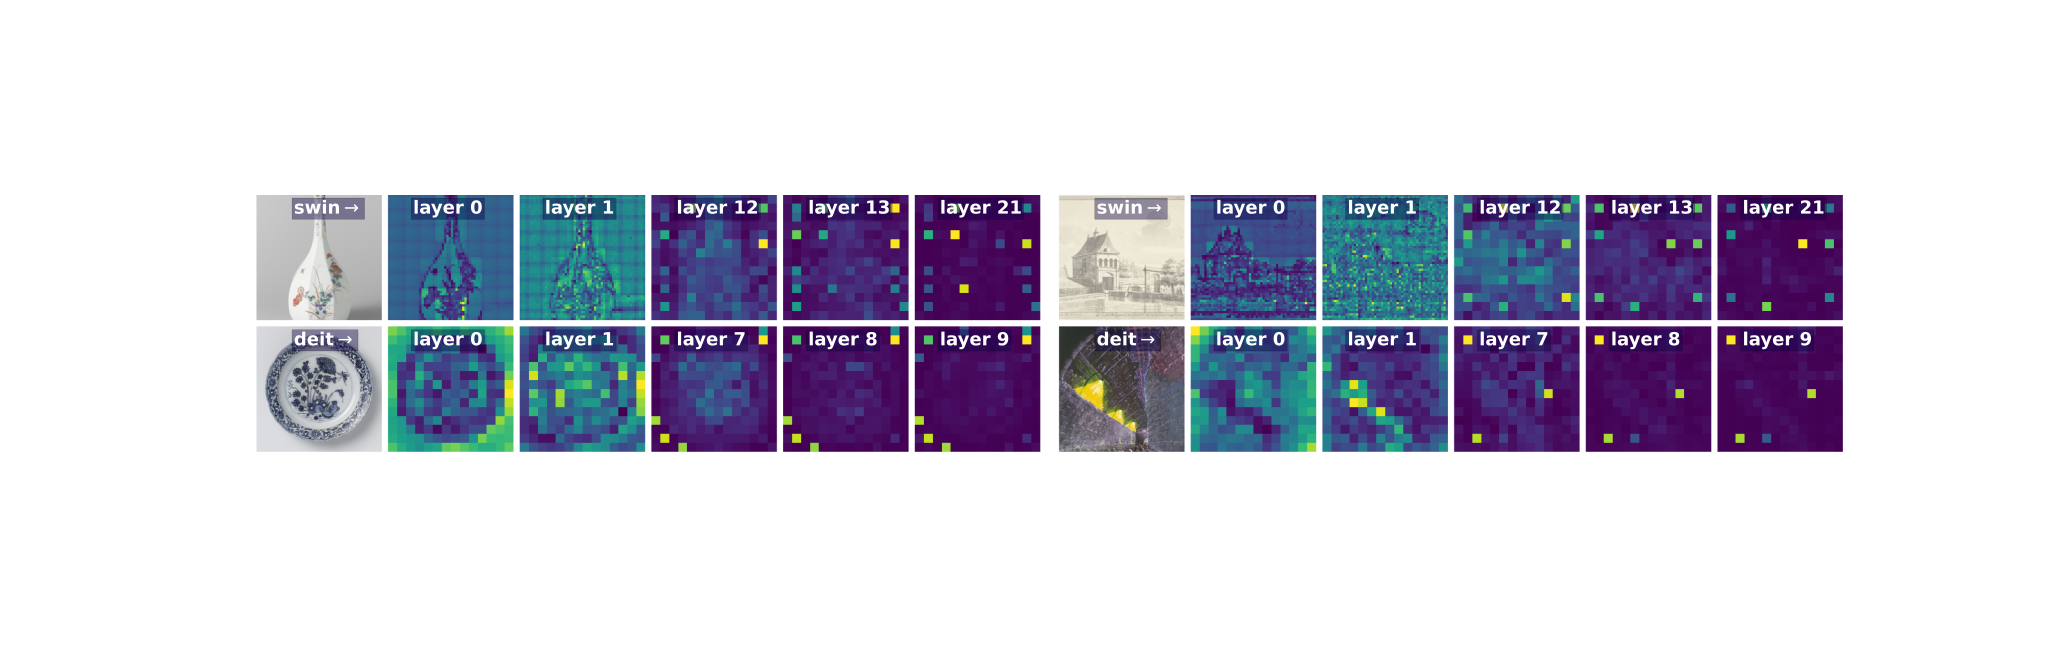
\includegraphics[width=\textwidth]{img/layers.png}
    \caption{Attention layers of successively deeper transformer blocks.}
    \label{results:img:layers}
\end{figure*}

\begin{figure*}[tb]
    \centering
    \begin{subfigure}{0.49\textwidth}
    \includegraphics[width=8cm]{img/img005_salience.png}
    \caption{Dish}
    \label{results:img:sal:dish}
    \end{subfigure}
    \begin{subfigure}{0.49\textwidth}
    \includegraphics[width=8cm]{img/img011_salience.png}
    \caption{Picture}
    \label{results:img:sal:dish}
    \end{subfigure}
    \caption{Examples of saliency maps for different models.}
\end{figure*}
